\chapter{Hybridní hry}
Hybridní hry kombinují jak prvky fyzické, tak digitální. Jedná se o hry, které mají jakékoliv napojení na technologii, ať už je to elektronické bankovnictví ve hře Monopoly Super Electronic Banking, či čtení příběhu a směrování dalšího postupu hráčů pomocí internetových stránek, ale stále se odehrávají ve fyzickém světě. Podobná spojení vyústí ve zcela nové herní zážitky, které si hráči mohou vyzkoušet.

\section{Vývoj hybridních her}
První hybridní hry se začaly formovat již na začátku 20. století, kdy se začaly objevovat první hry s elektrickými prvky. Tyto hry byly většinou jednoduché elektrické obvody, které hráč propojoval pro různé efekty. V průběhu času se tyto hry stávaly složitějšími a začaly se objevovat hry, které využívaly počítačové technologie. Hybridní hry mohou být kategorizovány do několika skupin, které se liší podle toho, jakým způsobem technologie využívají.

\subsection{Stolní hry s vlastním zařízením}
Mezi takovéto hry patří již výše zmíněný Monopoly Super Electronic Banking, který obsahuje elektronické bankovnictví, nebo známá hra Operation, ve které se nesmíte dotknout kovových částí na hrací desce, jinak se rozezní siréna. 

\begin{figure}[H]
    \centering
    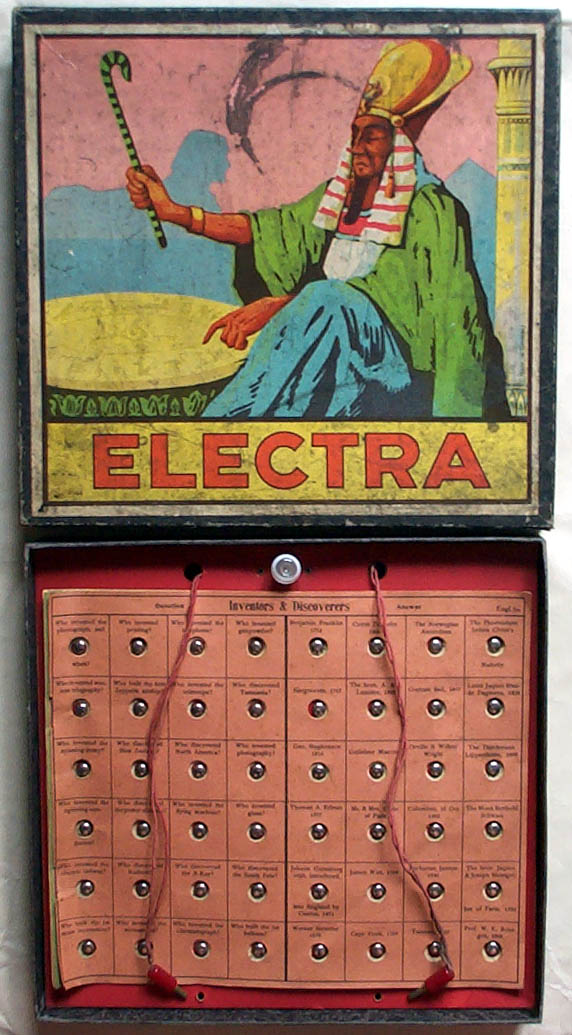
\includegraphics[width=0.3\textwidth]{resources/figures/electra.jpg}
    \caption{Hra Electra, první hybridní hra.\cite{history_of_hybrid_games}}
    \label{fig:electra}
\end{figure}

Tato kategorie hybridních her je rozhodně nejstarší. První hrou využívající elektrického proudu, a tudíž zařazenou do hybridních her, je hra Electra (původním názvem Lichtra). Jedná se o jednoduchou kvízovou hru, která vyšla už v roce 1910 v Německu a byla vytvořena společností Sala Games. Hra obsahovala jednoduchý elektrický obvod, který se uzavřel, pokud hráč odpověděl správně. Po této hře následovala dlouhá éra her, jejichž elektronika také spočívala pouze v propojení jednoho, či několika málo obvodů.\cite{history_of_hybrid_games, boardgames_with_apps}

Další zmínku ve vývoji her v této kategorii si zasloužila hra Voice of the Mummy, která vyšla v roce 1971. Hra měla v herním plánu zabudovaný přehrávač, který měl simulovat hlas mumie, která při přejití určitých herních polí hráčům určovala další postup.\cite{voice_of_the_mummy}

První hrou, která ve svém designu používala počítačové zařízení byla francouzská hra Simulateur JR10, která vyšla roku 1972. Jednalo se bitevní hru, ve které hráči ovládali různé jednotky. Při střetu jednotek se do počítače vložil děrný štítek s odpovídajícími jednotkami a počítač podle naprogramovaných kritérií náhodně určil výsledek střetu.\cite{simulateur_jr10}

\begin{figure}
    \centering
    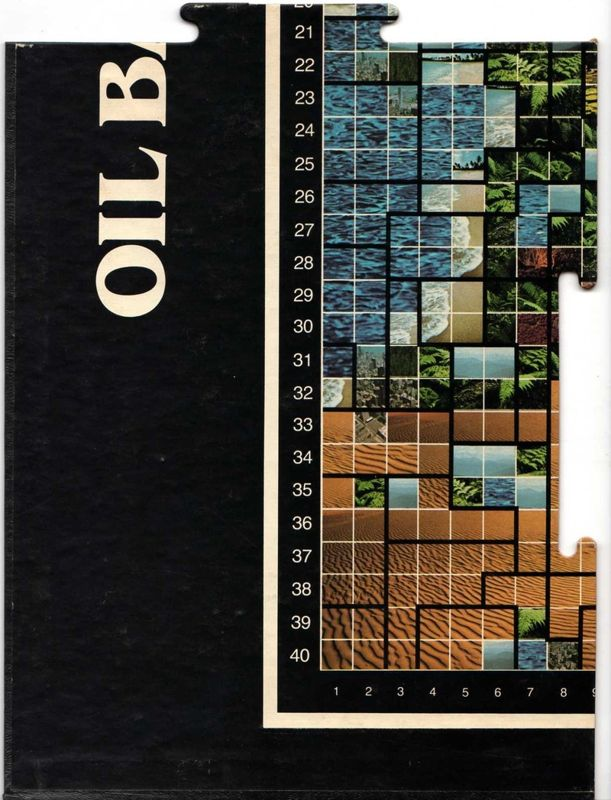
\includegraphics[width=0.35\textwidth]{resources/figures/oil_barons.jpg}
    \caption{Část herní desky Oil Barons.\cite{oil_barons}}
    \label{fig:oil_barons}
\end{figure}

\subsection{Stolní hry s počítačovými aplikacemi}
V roce 1983 byla společností Epyx vydána hra Oil Barons. Jednalo se o počítačovou hru, která šla spustit na zařízeních DOS, Apple II a Commodore 64. Její součástí byla fyzická hrací deska a několik herních tokenů. Samotný program měl za úkol simulovat náhodné výsledky a udržovat stav hry.\cite{oil_barons}

\section{Vybrané hybridní hry}
Následující hry jsem vybral jako příklady a inspiraci pro svou práci. Jedná se o stolní hry, které nějakým způsobem využívají právě internetových aplikací pro umocnění herního zážitku.

První z těchto her je Forgotten Waters (českým názvem Na vlnách neznáma). Jedná se o výpravnou RPG hru, která používá aplikaci jako nástroj pro vyprávění herního děje a k zaznamenávání hráčských rozhodnutí, díky čemuž hra dokáže dynamicky reagovat. Aplikace dále udává životy a statistiky nepřátel, slouží k výběru dějové linky a v neposlední řadě přispívá k zážitku hráčů pomocí namluvených scén. Tato aplikace je oficiální součástí dané hry a nelze ji bez ní hrát.

Dále bych chtěl uvést hru s názvem Gloomhaven, pro kterou, na rozdíl od hry předešlé, není aplikace potřebná, a dokonce momentálně neexistuje ani žádná oficiální. Hra samotná obsahuje velké množství různých karet, tokenů a dalších věcí, které, seč jsou pro hru samotnou podstatné, ji zbytečně protahují a komplikují. Z tohoto důvodu vzniklo pro tento titul hned několik pomocných aplikací, které se tyto problémy snaží řešit. Většina z nich si je velice podobná jak funkčností, tak vzhledem, jelikož vycházejí ze stylu samotné stolní hry.